\documentclass[a4paper]{article}
\usepackage{ucs}  % unicode
\usepackage[utf8x]{inputenc}
% \usepackage[T2A]{fontenc}
% \usepackage[bulgarian]{babel}
\usepackage{graphicx}
% \usepackage{fancyhdr}
% \usepackage{lastpage}
\usepackage{listings}
\usepackage{amsfonts}
\usepackage{amsmath}
% \usepackage{fancyvrb}
% \usepackage[usenames,dvipsnames]{color}
% \setlength{\headheight}{12.51453pt}

%\pagestyle{fancy}
%\fancyhead{}
%\fancyfoot{}

% \cfoot{\thepage\ от \pageref{LastPage}}

% \addto\captionsbulgarian{%
%   \def\abstractname{%
%     Цел на проекта} %\cyr\CYRA\cyrs\cyrt\cyrr\cyra\cyrk\cyrt}}%
% }

% Custom defines:

% TODO remove colorlinks before printing
% \usepackage[unicode,colorlinks]{hyperref}   % this has to be the _last_ command in the preambule, or else - no work
% \hypersetup{urlcolor=blue}
% \hypersetup{citecolor=PineGreen}

\def\d{\mathrm{d}}

\begin{document}

\title{High Level Computer Vision - Exercise 5}
\author{Zornitsa Kostadinova \\ Iskren Ivov Chernev}
\maketitle

\section*{Question 1}
\subsection*{b}
We experimented with the following parameters:
\begin{eqnarray*}
\sigma_1 &=& 5 \\
\sigma_2 &=& 5 \\
C &\in& \{ 0.1, 1, 10^2, 10^4, 10^6 \} \\
\end{eqnarray*}

The margins reported by the SVM were respectively

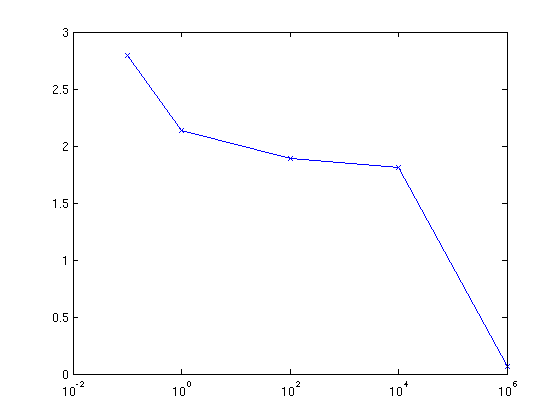
\includegraphics[scale=0.5]{margin_vs_c.png}

\begin{tabular}{|c|c|}
\hline
C   & margin \\ \hline \hline
$ 0.1 $ & $ 2.790273 $ \\
$ 1 $ & $ 2.134947 $ \\
$ 10^2 $ & $ 1.889752 $ \\
$ 10^4 $ & $ 1.807063 $ \\
$ 10^6 $ & $ 0.061729 $ \\ \hline
\end{tabular}

It is clear that the margin decreases exponentially as the constant $ C $ increases.

\end{document}
